% !TEX encoding = UTF-8 Unicode
% !TEX program = xelatex
% !BIB program = biber
% !TEX TS-program = xelatex
% !BIB TS-program = biber
%%
%%  本模板方式编译: XeLaTeX + biber
%%
%%  注意: 在改变编译方式前应先删除 *.toc 和 *.aux 文件
%%
\documentclass[12pt,openright]{book}

% 引入NKThesis包
\usepackage[emptydoublepage]{NKThesis}   % 中文
%\usepackage[emptydoublepage,English]{NKThesis} % 英文

% 其它包按需添加
\usepackage{hyperref}
\usepackage{bm}
\usepackage{amsmath}
\newtheorem{myDef}{定义}
\usepackage{float}
\usepackage{graphics}
\usepackage{algorithm}
\usepackage{algorithmicx}
\usepackage{algpseudocode}
%\usepackage[linesnumbered,ruled,vlined]{algorithm2e}
\usepackage{setspace}
\usepackage{multirow}
\usepackage{longtable}
\usepackage{subfigure} 
\renewcommand{\algorithmicrequire}{\textbf{输入:}}
\renewcommand{\algorithmicensure}{\textbf{输出:}}
%\renewcommand{\algorithmcfname}{算法}
% 参考文献
\addbibresource{nkthesis.bib}
% 图片文件夹
\graphicspath{{image/}}

\includeonly{
	./tex/abstract,
	./tex/introduction,
	./tex/relatedwork,
	./tex/method1,
	./tex/method2,
	./tex/discussion,
	./tex/summary,
	./tex/references,
	./tex/appendices,
	./tex/acknowledgements,
	./tex/resume
}
\begin{document}

%%%%%%%%%%%%%%%%%%%%%%%%%%%%%%%%%%%%%%%%%%%%%%%%%%%%%%%%%%%%%%%%%%%%%%%%%%%%%%%%
%  设置基本信息
%  注意:  逗号`,'是项目分隔符. 如果某一项的值出现逗号, 应放在花括号内, 如 {,}
%%%%%%%%%%%%%%%%%%%%%%%%%%%%%%%%%%%%%%%%%%%%%%%%%%%%%%%%%%%%%%%%%%%%%%%%%%%%%%%%
\NKTsetup{
	% 封面设置
	论文题目(中文) = 一种基于近边界数据的模型所有权推断方法研究,
	副标题         = ,
	论文题目(英文) = Research on Model Ownership Inference Based on Near-boundary Data,
	论文作者       = 杨宗稳,
	学号           = 2120200439,
	指导教师       = 蒲凌君副教授,
	申请学位       = 工学硕士,
	培养单位       = 南开大学,
	学科专业       = 计算机科学与技术,
	研究方向       = 模型的知识产权保护,
	答辩委员会主席 = {},
	评阅人 = {},
	中图分类号     = ,
	UDC            = ,
	学校代码       = 10055,
	论文完成时间   = 二〇二三年四月,
	% 保密设置
	密级           = 公开,	% 公开 | 限制 | 秘密 | 机密, 若为公开, 不填以下三项
	非公开论文编号 = ,
	保密期限       = ,
	审批表编号     = ,
	% 其他信息
	批准日期       = ,
	答辩日期       = ,
	论文类别       = 学历硕士, % 博士 | 学历硕士 | 专业学位硕士 | 同等学力硕士
	院/系/所       = 计算机学院,
	联系电话       = 13102257615,
	Email          = yzw@mail.nankai.edu.cn,
	通讯地址(邮编) = 300000,
	备注           = {},
}

%%%%%%%%%%%%%%%%%%%%%%%%%%%%
% 论文开始部分
%%%%%%%%%%%%%%%%%%%%%%%%%%%%
% 摘要
% !TeX root = ../main.tex
% -*- coding: utf-8 -*-


\begin{zhaiyao}

深度神经网络(Deep Neural Network, DNN)训练代价昂贵是导致模型知识产权保护问题逐渐被重视的原因。近年来,模型盗窃行为时常出现,不法分子对DNN模型非法复制,派生和发布的行为都严重侵犯了模型所有者的知识产权。许多研究者受到传统数字媒体水印的启发,从而设计模型水印和指纹用于验证模型所有权。然而,歧义性声明等攻击手段被用于破解模型水印和指纹,这对模型所有权验证工作造成了挑战。因此,需要设计一种知识产权保护方法能够解决上述问题。本文通过相关工作的调研,分析目前知识产权保护方法存在的难点与挑战,提出了一种基于近边界数据的模型所有权推断方法,主要工作如下:

1)揭示了当前DNN模型所有权验证方案的脆弱性并确认了数据驱动推断模型所有权的有效性。模型水印和模型指纹的方法通常用是检测嵌入的水印或者通过特定触发集来验证所有权,这种方式在面对歧义攻击击等强攻击时,并不具备很强的鲁棒性。DNN模型通过数据集训练,所以不管是源模型还是其派生出来的模型,总会包含一定数据中的知识,本文确认了数据驱动推断模型所有权方法的有效性。

2)提出了利用对抗性样本构造近边界数据以抵御模型窃取攻击。对抗性样本一般位于模型分类边界上并且相较于其他不相关的模型,对抗性样本可以更好的转移到从原始模型派生出的模型上。因此,本文利用对抗性样本构造了近边界数据来推断模型所有权,抵御模型窃取攻击。

3)设计了基于DCGAN的近边界数据生成器和提出了一种损失函数用以微调源模型的目标分类边界,增加推断模型所有权的置信度。为了防止近边界数据被轻易复制,本文使用DCGAN的生成器生成我们私有的近边界数据。在此基础之上,重新设计了模型损失函数微调源模型,在保持DNN模型性能的情况下,以95\%以上的置信度成功推断模型所有权。

4)本文在三个公开数据集上对本文提出的方法做了详细的测试,实验结果证明了基于近边界数据推断模型所有权的有效性和鲁棒性


\end{zhaiyao}



\begin{guanjianci}
知识产权保护;所有权推断;近边界数据;深度神经网络;生成对抗网络
\end{guanjianci}



\begin{abstract}

Deep Neural Network(DNN) training is expensive, which is why the issue of model intellectual property protection has been increasingly emphasized. In recent years, model theft has been occurring frequently, with malicious actors illegally copying, deriving, and releasing DNN models, which seriously violates the intellectual property of the model owners. Many researchers have been inspired by traditional digital media watermarks and have designed model watermarks and fingerprints to verify model ownership. However, attack methods such as ambiguity declarations have been used to break model watermarks and fingerprints, posing a challenge to model ownership verification. Therefore, a method for protecting intellectual property needs to be designed to address these issues. This paper analyzes the difficulties and challenges of current methods for protecting intellectual property through related work, and proposes a model ownership inference method based on near-boundary data. The main contributions of this work are as follows:

1)We reveal the vulnerability of current DNN model ownership verification schemes and confirm the effectiveness of data-driven inference of model ownership. The methods of model watermark and model fingerprint are usually used to detect embedded watermarks or to verify ownership through specific trigger sets. However, these methods do not have strong robustness in the face of strong attacks such as ambiguity attacks. Since DNN models are trained on a dataset, both the source model and its derivatives will contain some knowledge from the data. This paper confirms the effectiveness of data-driven inference of model ownerships.
 
2)We propose the use of adversarial samples to construct near-boundary data to resist model theft attacks. Adversarial samples are generally located on the model classification boundary and can be better transferred to models derived from the original model compared to other unrelated models. Therefore, this paper uses adversarial samples to construct near-boundary data for ownership inference and to resist model theft attacks.

3)We design a near-boundary data generator based on DCGAN and propose a loss function to fine-tune the target classification boundary of the source model to increase the confidence of ownership inference. In order to prevent near-boundary data from being easily copied, this paper uses a DCGAN generator to generate private near-boundary data. On this basis, the model loss function is redesigned to fine-tune the source model, successfully inferring model ownership with over 95\% confidence while maintaining DNN model performance.

4)We conduct detailed tests on three public datasets to verify the effectiveness and robustness of the proposed method based on near-boundary data for model ownership inference. The experimental results demonstrate  the effectiveness and robustness of ownership inference based on near-boundary data.

\end{abstract}



\begin{keywords}
Intellectual property protection; Ownership inference; Near-boundary data; Deep neural network; Generative adversarial network
\end{keywords} 
% 论文目录
\tableofcontents

% 列出图表目录,如果需要可取消注释
% \listoffigures

%%%%%%%%%%%%%%%%%%%%%%%%%%%%
% 论文主体章节
%%%%%%%%%%%%%%%%%%%%%%%%%%%%
% !TeX root = ../main.tex
% -*- coding: utf-8 -*-

\chapter{绪论}
\label{1}


\section{研究背景与意义}

机器学习的发展

模型知识产权问题描述

模型知识产权相关研究

\section{相关研究现状}

研究问题

研究现状

\section{本文主要工作}

揭示\cite{maini2021dataset}现有问题,确认数据驱动推断所有权的有效性

利用对抗性样本抵御模型窃取

基于DCGAN生成私有数据

广泛实验验证有效性

\section{本文组织架构}

第一章

第二章

第三章

第四章

第五章

第六章
% !TeX root = ../main.tex
% -*- coding: utf-8 -*-


\chapter{技术背景} 
\label{2}

引言

\section{深度神经网络及相关术语}

人工神经网络是一种类似于人类大脑生物神经系统的信息处理模型,它由许多相互连接的神经元(网络中的节点)组成,这些神经元都可以向其他神经元发送信号。一般的神经网络由输入层,隐藏层和输出层组成,如图\ref{深度神经网络结构图}所示,如果一个神经网络有多个隐藏层,那么这个神经网络就被称为深度神经网络。DNN的隐藏层一般由卷积层,池化层,全连接层,Dropout层和Softmax层构成,数据输入输入层后,会经过每一层,每层提取的抽象特征会作为下一层的输入,最终由输出层输出。

\begin{figure}[htbp]%%图,[htbp]是浮动格式
	\centering
	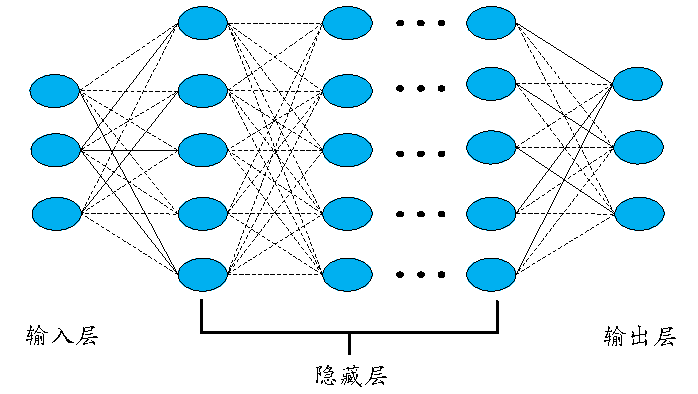
\includegraphics[width=11cm,height=7cm]{深度神经网络结构.pdf}
	%	\centerline{原始样本}
	\setlength{\abovecaptionskip}{5mm} %图片标题与图片距离
	\caption{深度神经网络结构图}
	\label{深度神经网络结构图}
\end {figure}

DNN可以看作是将一组输入变量转化为一组输出变量的非线性数学函数。每个神经元都有对应的权重和偏置参数,控制着输入的精确转化,这些参数在反向传播的过程中,通过损失函数和梯度下降算法来更新。确定这些参数的过程称为DNN模型的学习或者训练,并且需要大量的计算资源,然而权重一旦确定,DNN模型就可以快速的处理相似类型的新数据,识别并提取海量数据中的复杂特征。

以下是本文中涉及到DNN知识产权保护领域中的相关术语:

\begin{enumerate}
	\renewcommand{\labelenumi}{\theenumi)}
	\item 源模型。源模型也称作目标模型,是指模型所有者在私有或公共数据集上,消耗大量计算资源和人力资源训练出的高性能DNN模型,可能因学术研究放置在开源社区,或者作为商用给用户提供远程API。
	\item 可疑模型。可疑模型是指该模型可能是通过模型窃取攻击方法从源模型派生出来的模型,判断一个可疑模型是否是从源模型派生是模型知识产权保护领域的主要目标。
	\item 白盒模式。白盒模式是指能够获得DNN模型的所有知识,包括训练集,训练方式,模型参数,模型结构等。
	\item 黑盒模式。黑盒模式指不清楚模型内部参数,但可以通过模型提供的API获得指定输入的输出。
\end{enumerate}



\section{对抗性攻击}

\subsection{对抗性样本}
 
对抗性样本的概念是Szegedy等人\cite{szegedy2013intriguing}提出的。这篇文章中指出,通常情况下,一个良好性能的DNN模型具备很好的泛化能力,对输入的随机微小扰动具有鲁棒性,因此小扰动不应该改变图像的预测类别。然而,对图像添加特定的非随机扰动,使得损失函数的值增大,可以任意改变DNN模型的预测结果。这种人类肉眼上难以察觉但可以使模型输出错误类别的样本称为对抗性样本。 

用$f:R^m \rightarrow {1,2,...,n}$表示将一张图片映射为$n$个标签的DNN分类器,对一个正常样本$x \in R^m$以及一个错误标签$l$,目标是找到一个最小的扰动$\delta$,使得分类器将样本$x$错误分类为$l$,如式\ref{eq:1}所示:
\begin{equation}
	\label{eq:1}
	\begin{split}
	&min\parallel \delta \parallel_2, \\
	 &s.t. \ f(x + \delta) = l,\ x + \delta \in [0,1]^m
	\end{split}
\end{equation}
其中叠加了扰动的$x +\delta$即为一个对抗性样本。\ref{eq:1}这种方式通常用在黑盒的场景下,仅根据DNN分类器的输出进行扰动$\delta$的调整。
 
 在白盒场景下,由于知道模型的所有知识,可以根据这些信息来寻找对抗性样本,通常利用DNN分类器的损失函数来寻找对抗性样本。
 
 用$f:R^m \rightarrow {1,2,...,n}$表示将一张图片映射为$n$个标签的DNN分类器,对一个正常样本$x \in R^m$以及它对应的正确标签$y$,目标是找到一个足够小小的扰动$\delta:\delta \leq \gamma$,使得加上扰动后的样本输入DNN模型后,损失函数$L$达到最大值,如式\ref{eq:2}所示:
 \begin{equation}
 	\label{eq:2}
 		\delta = arg \mathop{max} \limits_{\delta \leq \gamma} L(f(\theta, x + \delta), y)
\end{equation}
其中$\theta$是分类器$f$的参数,$x + \delta$是一个扰动后的对抗性样本。
 
 \subsection{对抗性攻击的类别}

对抗性攻击技术是指生成对抗性样本的方法,不同的方法生成对抗性样本的效率,质量也不相同。根据方式的不同,可以分为以下几类:

\begin{enumerate}
	\renewcommand{\labelenumi}{\theenumi)}
	\item 白盒攻击与黑盒攻击。白盒攻击指敌手知道DNN模型的参数和内部结构等信息,利用这些信息发起的攻击。黑盒攻击指敌手仅根据模型的输入输出来发起攻击。
	\item 有目标攻击和无目标攻击。有目标攻击指对抗性样本的预测类别为敌手指定的类别,例如将一张牛的图片识别为羊,而不能是其他类别,常采取的方式是向各个方向搜索扰动来最大化DNN模型预测特定类上的可能性。无目标攻击指添加扰动来改变原始预测类别,对具体分类类别不做要求。通常来说有两种攻击方式,一种是最小化DNN模型预测正确类的可能性,一种是进行多次不同类别的的有目标攻击,然后在多个对抗性样本中选取扰动最小的。
	\item 单步攻击和迭代攻击。单步攻击指通过一次添加扰动生成对抗性样本,迭代攻击指通过多次迭代添加微小扰动来生成对抗性样本。通常来说迭代攻击的成功率较高,但是相应的算法复杂度更高,效率较低。
	\item 个体攻击和普适性攻击。个体攻击指针对每个样本都需要重新生成扰动,普适性攻击指找到一个通用的扰动,对数据集中的一类数据都叠加该扰动,普适性攻击效率较高,但是寻找通用扰动的难度较大。
\end{enumerate}

\section{生成对抗网络}

Goodfellow等人\cite{goodfellow2014generative}第一次提出了生成对抗网络(Generative Adversarial Network, GAN),GAN由一个生成器和一个判别器构成,

\begin{figure}[htbp]%%图,[htbp]是浮动格式
	\centering
	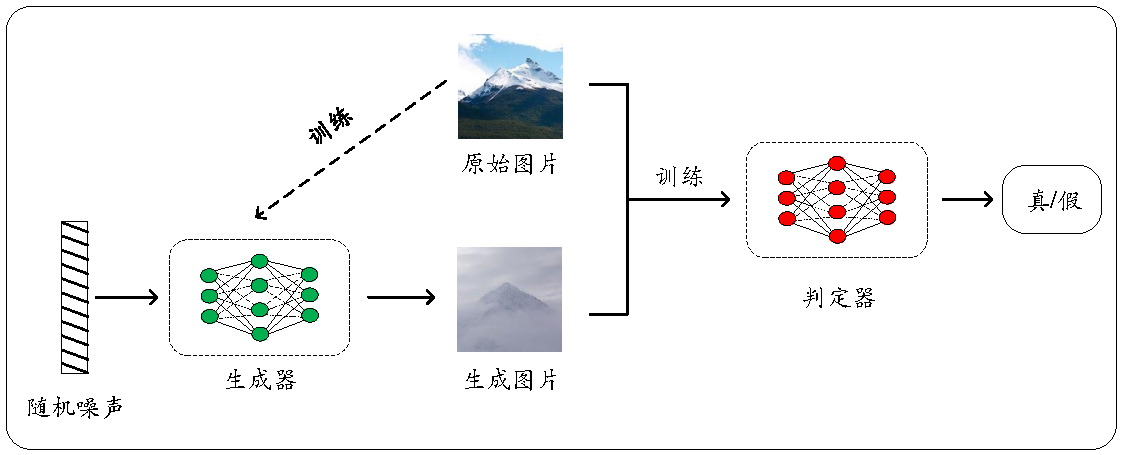
\includegraphics[width=14.5cm,height=7cm]{生成对抗网络结构.pdf}
	%	\centerline{原始样本}
	\setlength{\abovecaptionskip}{5mm} %图片标题与图片距离
	\caption{生成对抗网络结构图}
	\label{生成对抗网络结构图}
\end {figure}






\section{深度神经网络模型窃取攻击}

深度神经网络模型窃取攻击相关概念


\section{深度神经网络模型的知识产权保护}


深度神经网络模型的知识产权保护相关概念


\section{本章小结}


小结

% !TeX root = ../main.tex
% -*- coding: utf-8 -*-

\chapter{基于生成对抗网络特征提取的近边界数据研究}\label{3}

DNN分类器可以由其分类边界唯一的表示,本章将讨论DNN模型分类边界的具体表示方法,给出量化的分类边界距离定义,研究对抗性样本在源模型和派生模型上的可转移性以及生成近边界对抗性样本的方法和阐述DCGAN私有化近边界数据的详细过程。

\section{近边界对抗性样本}

DNN分类器的主要目标是对输入数据样本进行分类,因此,一个DNN分类器的特征通常由其决策模式和分类边界决定。分类器的分类边界是一个抽象的概念,我们无法直接描述它,但可以根据分类器的决策结果来间接的反应分类边界。下面给出分类器分类边界的定义:

\begin{Definition}[分类边界]
	\label{def:1}
	给定一个数据样本$x$,如果数据样本$x$满足$g_i(x) = g_j(x)$,其中$i \neq j $并且$min(g_i(x), g_j(x)) > \mathop{max} \limits_{k \neq i, j}g_k(x)$,$g_k(x)$代表数据样本$x$被决策为类别$k$的概率,那么称数据样本$x$位于类别$i$和$j$的分类边界上。
\end{Definition}

注意,分类边界是DNN分类器的特征,是客观存在的,和我们是否能直接找到这样的数据点并不相关。因此,如何有效的获取分类边界或其附近的数据样本点,是本文方法要解决的问题之一。

模型窃取攻击是一种通过攻击目标模型并构建一个相似但不完全一样的模型来非法获取模型的技术。在这种攻击中,攻击者通常会对源模型进行修改,以便逃避模型所有者的检测。这些修改会导致源模型的分类边界发生变化,所以通常无法保证位源模型分类边界上的数据样本样本依旧位于可疑模型分类边界上。

对抗性样本是一类特殊的数据样本,它可以使得DNN模型输出异常的结果。虽然我们可以找到位于源模型分类边界上的对抗性样本,但是在经过修改的可疑模型中,因为分类边界的偏移,无法保证对抗性样本依然位于其分类边界上。因此,直接利用分类边界来作为模型指纹是脆弱的,因为模型修改会影响分类边界。

为了解决这个问题,与分类边界的思想类似,本文提出了一个鲁棒性更强的近边界数据概念。下面给出本文近边界数据的定义:

\begin{Definition}[近边界数据]
	\label{def:2}
	给定一个数据样本$x$,一个阈值$\theta$,如果数据样本$x$满足$\vert g_i(x) - g_j(x) \vert \leq \theta$,其中$i \neq j $并且$min(g_i(x), g_j(x)) \geq \mathop{max} \limits_{k \neq i, j}g_k(x)$,$g_k(x)$代表数据样本$x$被决策为类别$k$的概率,则数据样本$x$被称为近边界数据。
\end{Definition}

近边界数据是指那些非常接近分类边界的数据样本,与位于分类边界上的数据样本类似,这些样本对模型的决策边界有重要的影响,因为它们能够揭示模型在边界附近的行为。由于近边界数据不要求样本完全位于分类边界上,因此即使模型分类边界发生偏移,仍然可以衡量数据近边界性。所以相对于直接使用分类边界来作为模型指纹,近边界数据在面对模型窃取攻击时有着更强的鲁棒性。

如图\ref{近边界数据示意图}所示,近边界数据位于DNN分类器的分类边界附近,其他数据的分布则离分类边界较远。判定是否为近边界数据由定义\ref{def:2}中的阈值$\theta$决定,当$\theta$较小时,近边界数据样本表现为更加靠近模型分类边界。

\begin{figure}[htbp]%%图,[htbp]是浮动格式
	\centering
	\setlength{\abovecaptionskip}{5mm} %图片标题与图片距离
	\vspace{-2mm}
	\setlength{\belowcaptionskip}{-3mm} %调整图片标题与下文距离
	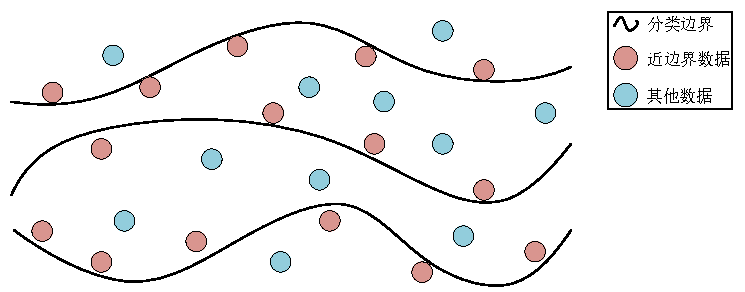
\includegraphics[width=0.9\linewidth]{近边界数据示意图.pdf}
	\caption{近边界数据示意图}
	\label{近边界数据示意图}
	%	\vspace{-3mm}  %调整图片标题与下文距离,与\setlength{\belowcaptionskip}{-3mm}等效。
	\end {figure}
		
相较于其他不相关的模型,对抗抗性样本可以更好的从源模型转移到其派生出的模型上。与对抗性样本类似,近边界数据也可以随着源模型转移,也就是说数据的近边界特性在派生模型上得到保留,详细的测试结果在\ref{5}\ref{5.3}中。在下一节中,我们将讨论如何生成所需的近边界对抗性样本。

\section{生成近边界对抗性样本}\label{3.2}

尽管近边界数据在模型的知识产权保护中表现出显著的效果,但是在实践中,获得一定规模的近边界数据样本仍然是一个具有挑战性的任务。这主要是由于自然的近边界数据在样本空间中的占比非常低,甚至可以被忽略不计,因此如何得到一定规模的近边界数据样本仍然是一个难题。

根据最近的一些研究\cite{cao2021ipguard},对抗性样本通常被用于确定分类器的分类边界。具体而言,对抗性样本有两个分类:原始分类和目标分类。其中,原始分类是指该样本不经过特殊处理的原始分类结果,目标分类是对原始样本添加微小噪声后的分类结果。对抗性样本是通过向原始数据添加小量扰动或干扰来生成的,这些扰动通常很难被人眼察觉,但却足以改变DNN模型的分类结果。

如图\ref{原始样本与对抗性样本对比}所示,对抗性样本对分类边界的跨越体现在,在视觉上,对抗性样本和原始样本几乎没有差别,但是分类结果却完全不同,在有目标攻击的情况下,甚至可以人为的指定目标分类。如在图\ref{原始样本与对抗性样本对比}中,原始样本的类别为石柱,对抗性样本却被分类器识别为高塔。

\begin{figure}[htbp]%%图,[htbp]是浮动格式
	\setlength{\abovecaptionskip}{3mm} %图片标题与图片距离
	\vspace{-2mm}
	\setlength{\belowcaptionskip}{-3mm} %调整图片标题与下文距离
	\subfigure[原始样本]{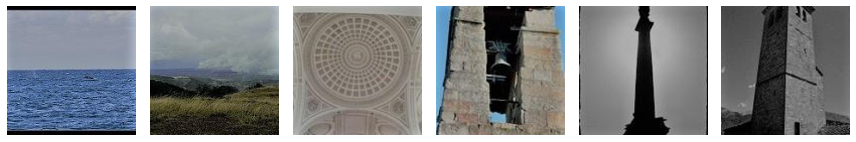
\includegraphics[width=1\linewidth]{原始样本.pdf}}
	\subfigure[对抗性样本]{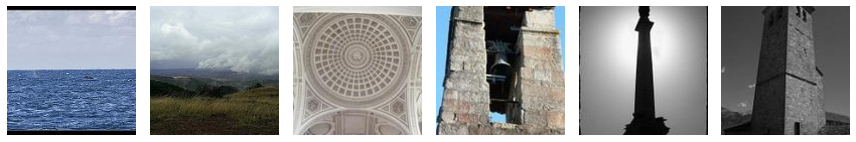
\includegraphics[width=1\linewidth]{对抗性样本.pdf}}
\caption{原始样本与对抗性样本的对比}
\label{原始样本与对抗性样本对比}
\end {figure}

对抗性样本会对分类边界进行跨越,我们认为该特征可以帮助获得较多的近边界数据。具体来说,我们将生成大量的对抗性样本,并从中挑选合适的近边界数据。因此,本文测试了几种常见的生成对抗性样本的方法,以帮助我们更好的构建近边界数据。因为我们希望数据样本尽可能靠近分类边界,因此在测试过程中,不同方法的优劣取决于生成对抗性样本到分类边界距离的远近,距离近者更优。

为了更好的衡量数据样本到分类边界的距离,在定义\ref{def:2}的基础上,下面给出量化的分类边界距离定义:

\begin{Definition}[分类边界距离]
	\label{def:3}
	给定一个数据样本$x$,它到分类边界的距离$distance = \vert g_i(x) - g_j(x) \vert$,其中$i \neq j $并且$min(g_i(x), g_j(x)) \geq \mathop{max} \limits_{k \neq i, j}g_k(x)$,$g_k(x)$代表数据样本$x$被决策为类别$k$的概率。
\end{Definition}

根据定义\ref{def:3},以分类边界距离为衡量标准,下面分别对几种常见的生成对抗性样本的方法进行介绍与测试。


\noindent\textbf{Fast \ Gradient \ Sign \ Method(FGSM):}FGSM \cite{goodfellow2014explaining}是最经典的生成对抗性样本的方法之一,它是一种基于梯度构建对抗性样本的方法,属于无目标的攻击方式。只需要对原始样本添加一次微小的扰动$\eta$,如式\ref{eq:3.1},\ref{eq:3.2}所示,即可生成样本$x$的对抗性样本$\tilde{x}$,十分高效。

\begin{equation}
	 	\setlength\abovedisplayshortskip{-5mm}
%	 	\setlength\belowdisplayshortskip{4mm}
	\label{eq:3.1}
	\eta = \epsilon \cdot sign(\bigtriangledown_xJ(\theta,x,y^*))
\end{equation}
\begin{equation}
	\label{eq:3.2}
	\tilde{x} = clip(x + \eta)
\end{equation}

\noindent 其中$sign$是符号函数,$x$表示原始样本,$y^*$表示$x$的真实类别,$\theta$表示模型权重参数,$J$表示分类器损失函数,$\bigtriangledown_x$表示对原始样本$x$求偏导,$clip$函数是将样本投射回可行数据域,比如图像样本的像素点范围应该在$[0,1]$以内,$\epsilon$用来控制变化幅度大小。

FGSM 生成对抗性样本的速度非常快,但其结果非常依赖$\epsilon$的选择,因此探索不同的$\epsilon$是使用该方法的重点。

\noindent\textbf{Iterative \ Gradient \ Sign \ Method(IGSM):}IGSM\cite{kurakin2018adversarial}是FGSM的进阶版本,如式\ref{eq:3.3},\ref{eq:3.4}所示,与FGSM只进行一次扰动叠加不同,IGSM采用迭代的形式构造对抗性样本,每次叠加一个小扰动。这个过程持续到成功生成对抗性样本或者达到迭代次数上限为止。

\begin{equation}
	\setlength\abovedisplayshortskip{-5mm}
	\label{eq:3.3}
	\eta = \alpha \cdot sign(\bigtriangledown_xJ(\theta,x,y^*))
\end{equation}
\begin{equation}
	\label{eq:3.4}
	\tilde{x}_t = clip(\tilde{x}_{t - 1}  + clip_{\epsilon}(\eta))
\end{equation}

\noindent 其中$\alpha$是步长大小,$\tilde{x}_t$表示第$t$次迭代后的结果,$clip_{\epsilon}$是限定每次叠加的范围不超过$\epsilon$,其余参数含义与FGSM保持一致。

除此之外,我们还测试了FGSM的另一个进阶版本RFSGM\cite{tramer2017ensemble},RFSGM增加了扰动的多样性,可以更精细地生成对抗性样本。在实际结果中我们发现尽管FGSM生成对抗性样本速度非常快,但是对抗性样本距离分类边界的距离比较远。IGSM 和RFGSM 效果要比FGSM 好,但仍然没有达到我们的预期,生成的对抗性样本距离分类边界距离太远。在大量的测试中,我们发现CW能够生成大量位于分类边界附近的样本,具体的测试结果在\ref{5}\ref{5.2}中。

\noindent\textbf{Carlini \ and \ Wagner's \ methods(CW):}CW\cite{carlini2017towards}方法是一种有目标的攻击方式,同样是添加噪声到对抗性样本中,但其具有三种变体:CW-$L_0$,CW-$L_2$和CW-$L_{\infty}$,不同的变体使用不同的方法来衡量噪声的大小,其中CW-$L_2$在实验中生成对抗性样本的效果和生成效率相比其余两种变体较好,因此本文使用该方法作为生成对抗性样本的选择。具体而言,CW-$L_2$对于给定的初始样本,采用二分查找的方式来增大或减小式\ref{eq:3.7}中$c$,并且使用类似训练神经网络模型的方式来调整生成对抗性样本的其他参数。CW-$L_2$的损失函数和约束如式\ref{eq:3.5},\ref{eq:3.6},\ref{eq:3.7},\ref{eq:3.8}所示:

\begin{equation}
%	\setlength\abovedisplayshortskip{-8mm}
	\label{eq:3.5}
	Loss = Loss1 + Loss2 
\end{equation}
\begin{equation}
%	\setlength\abovedisplayshortskip{-8mm}
	\label{eq:3.6}
	Loss1 = D(x, x + \delta)
\end{equation}
\begin{equation}
%	\setlength\abovedisplayshortskip{-5mm}
	\label{eq:3.7}
	Loss2 = c \cdot f(x + \delta,target)
\end{equation}
\begin{equation}
%	\setlength\abovedisplayshortskip{-5mm}
%	\setlength\belowdisplayshortskip{-3mm}
	\label{eq:3.8}
	x + \delta \in [0,1]^m
\end{equation}

\noindent 其中$target$是生成对抗性样本的目标标签,$c$是惩罚因子,用于权衡$Loss2$的影响大小,算法通过二分查找来寻找合适的$c$。$Loss1$约束对抗性样本$x + \delta$和原始样本$x$尽可能相似,$Loss2$约束对抗性样本$x + \delta$的决策结果为目标标签,式\ref{eq:3.8}约束对抗性样本在正常的图像范围内。

根据定义\ref{def:3},数据样本$x$距离分类边界的距离是$distance = \vert g_i(x) - g_j(x) \vert$,本节的目标是生成的对抗性样本距离分类边界的距离尽可能近。我们在算法迭代过程中引入这一目标,以此改进算法迭代的过程,在使得生成对抗性样本更加靠近分类边界的同时,提高算法效率。具体而言,在迭代过程中,我们仅在$distance$变小时,更新距离参数和新生成的对抗性样本,并在$distance$小于等于预定的阈值$\theta$时,提前终止算法的迭代,具体的过程如算法\ref{alg:1}所示。

\begin{algorithm}[H] 
	\setstretch{1.2}
	\caption{改进的二分查找CW-$L_2$算法}
	\label{alg:1}
	\begin{algorithmic}[1]
		
		\Require 样本$x$;模型$M$;阈值$\theta$;二分次数$n$;迭代次数$iteration$;原始标签$r$;目标标签$t$
		\Ensure 近边界对抗性样本$x'$
		\State 参数初始化:$c\gets1$,$distance \gets 1$
		\For {$i=1,2,...,n$}
			\State $isSuccessAttack \gets false$
			\State $w \gets arctanh(x)$
			\State $w\_pert \gets zero\_like(w)$
			\For{$j=1,2,...,iteration$}
				\State $new\_img \gets tanh(w + w\_pert)$
				\State $new\_distance \gets \vert g_r(new\_img) - g_t(new\_img) \vert$
				\If{$new\_distance < distance$}
					\State $distance \gets new\_distance$
					\State $x' \gets new\_img$
					\State $isSuccessAttack \gets true$
				\EndIf
				\State 使用$Adam$更新$w\_pert$
			\EndFor
			\If{$isSuccessAttack == true$}
			\State 减小$c$
			\Else \State 增大$c$
			\EndIf 
			\If{$distance \leq \theta$} 
			\State $break$
			\EndIf
		\EndFor
		\State \textbf{return} $x'$
	\end{algorithmic}
\end{algorithm}

通过算法\ref{alg:1},我们已经可以生成大量位于分类边界附近的对抗性样本,即本文所需要的近边界数据。但是在这一阶段,我们只是在源模型的样本空间中挑选一部分数据作为初始样本添加微小噪声或扰动,针对性地生成了目标分类的对抗性样本。

在此阶段,源模型的训练和原始训练数据集均不受任何影响,防御者只需要针对性的生成对抗性样本即可。然而,近边界数据作为推断所有权的重要证据,直接生成对抗性样本也极易受到盗窃者的复制。因此,我们需要将生成的近边界数据私有化,防止盗窃者的模仿,具体操作将在下一节中给出。

\section{近边界数据私有化}\label{3.3}

因为现在大多数模型训练使用的数据都来源于公开的数据集,所以通过生成对抗性样本的方法构建近边界数据这一步骤也十分容易复现。因此我们需要从公开的训练数据中构建自己的私有化近边界数据,以防止模型所有者的近边界数据被轻易模仿,这是十分必要的,因为近边界数据是后续推断模型所有权的核心依据。

在本文中,我们希望可以通过训练一种模型学习上一节中生成的近边界对抗性样本的特征,并以此生成新的私有化近边界数据。这种新的数据从视觉上不一定和原始数据类似,但其原始的特征以及添加的噪声需要被学习,并根据提取到的特征生成的新样本对于源模型同样是近边界数据。因为本文用到的是图像样本,CNN可以很好的处理图像。因此,在本文中,我们设计了一种基于DCGAN\cite{radford2015unsupervised}的特征提取器,提取近边界数据的特征之后,使用生成器生成私有化的近边界数据。
%注意生成器以,$CW$-$L_2$生成的对抗性示例作为输入,并输出私有化后的近边界数据。

\begin{figure}[htbp]%%图,[htbp]是浮动格式
	\centering
	\setlength{\abovecaptionskip}{5mm} %图片标题与图片距离
%	\vspace{-2mm}
	\setlength{\belowcaptionskip}{-3mm} %调整图片标题与下文距离
	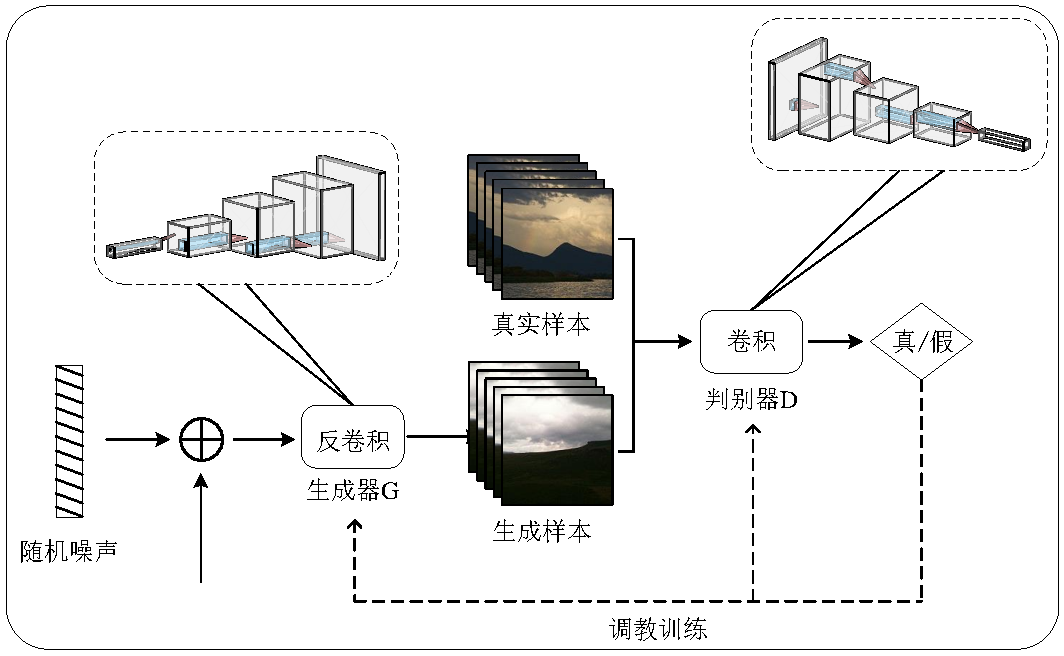
\includegraphics[width=1\linewidth]{DCGAN网络结构图.pdf}
	\caption{DCGAN网络结构图}
	\label{DCGAN网络结构图}
	%	\vspace{-3mm}  %调整图片标题与下文距离,与\setlength{\belowcaptionskip}{-3mm}等效。
	\end {figure}
	
如图\ref{DCGAN网络结构图}所示,DCGAN的大体结构与训练方式和普通GAN类似,主要变化是DCGAN将原始的GAN与CNN结合到一起,生成器$G$和判定器$D$都用CNN架构替换了原始GAN的全连接网络。得益于CNN对图像的强大处理能力,DCGAN极大提升了网络训练稳定性和生成样本的质量。具体而言,DCGAN主要是从网络架构上改进了原始的GAN,主要改进如下:

1)DCGAN的生成器和判别器均舍弃掉CNN的池化层,生成器使用反卷积层来还原图片,判别器保留CNN的整体架构,使用卷积层来提取图片特征。

2)在生成器和判别器中都使用Batch Normalization层,提升训练DCGAN模型稳定性的同时加速了训练。

3)生成器除最后一层使用Tanh激活函数外,其余层使用ReLU,判别器所有层均使用LeakyReLU,使模型可以更快的学习。

4)使用Adam优化器并调整了超参数,将学习率设置为0.0002,可以更好的学习到数据样本的特征。

我们希望DCGAN能够学习到尽可能多的近边界数据特征,以便更好的生成近边界数据。训练过程中,尝试修改DCGAN判定器的目标函数,在保留梯度的情况下,将其与源模型的结果相连,即使用源模型和判别器共同判定是生成数据还是原始数据。这种方式得到的训练结果在同样的生成规模下略微优于原始DCGAN生成的数据。然而,考虑到两者的效率,实际情况下生成的结果并无较大区别,所以本文采用原始的训练方式。训练DCGAN的具体流程如算法\ref{alg:2}所示。

\begin{algorithm}[!h] 
	\setstretch{1.2}
	\caption{训练DCGAN模型}
	\label{alg:2}
	\begin{algorithmic}[1]
		
		\Require 近边界数据$\tilde{D}$;批处理大小$batchsize$;训练轮次$epoch$;损失函数$Loss$
		\Ensure 训练好的DCGAN模型
		\State 参数初始化:$learning \ rate \gets 0.0002$,$real\_label \gets 1$,$fake\_label \gets 0$
		\For{$i=1,2,...,epoch$}
		\State 随机噪声$z \gets 100$ 
		\State $x' \gets G(z)$
		\State $Loss1 \gets Loss(D(x), real\_label)$  \Comment $x$是近边界数据样本
		\State $Loss2 \gets Loss(D(x'), fake\_label)$
		\State $Loss_D \gets Loss1 + Loss2$
		\State $Loss_G \gets Loss(D(x'), real\_label)$ \Comment 生成器希望$D(x') $接近$real\_label$
		\State 使用$Adam$优化器更新生成器$G$,判别器$D$的网络参数
		\EndFor
	\end{algorithmic}
\end{algorithm}

通过算法\ref{alg:2},完成训练DCGAN模型后,DCGAN的生成器便可以作为近边界数据特征提取器。训练过程中,通过生成器和判定器的相互博弈,生成器生成图像的特征分布会愈来愈接近原始近边界样本。训练收敛时,生成器已经学习到近边界数据的特征。我们可以通过生成器生成私有的近边界数据,这样的数据仍然具备近边界性,且可疑对手无法轻易获得。

DCGAN对图像数据有着很强的特征提取能力,生成器能够很好的学习近边界数据特征,使用生成器构建的近边界数据位于目标分类边界附近。但是相比于原始近边界数据,由于随机因素,生成的数据样本近边界性会弱于原始近边界数据,我们仍然希望近边界数据最大程度上靠近目标分类边界。因为近边界数据与目标分类边界的距离越近,推断模型所有权成功的可能性就越大。此外,生成的私有近边界数据虽然只被模型所有者拥有,但对于一些功能易被泛化的模型,经过模型窃取攻击后,由于模型被修改,数据的近边界特性仍有可能被泛化。

因此,为了解决上述问题,本文提出使用近边界数据微调源模型的目标分类边界,使生成的私有近边界数据更加靠近DNN模型分类边界。如式\ref{eq:3.4}所示,$Loss_{FT}$是针对目标分类边界的损失函数。

\begin{equation}
%	\setlength\abovedisplayshortskip{-3mm}
	\label{eq:3.9}
	Loss_{FT} = \frac{1}{n} \sum^{n}_{i = 1} (g_t(x_i') - g_s(x_i'))^2
\end{equation}

\noindent 其中$n$是该目标分类边界的近边界数据的数量,$x_i'$是生成的近边界数据,$g_t(\cdot)$和$g_s(\cdot)$分别表示目标分类概率和源分类概率。

$Loss_{FT}$本质是希望近边界数据更靠近目标分类边界,但是为了尽可能减小对原始模型精度的影响,不能直接使用该损失函数对源模型进行微调。受DCGAN训练过程的启发,我们使用源模型的损失函数$Loss_{FM}$与$Loss_{FT}$两者交替训练微调源模型,并将学习率设置为0.0001,在保持源模型精度的同时,使生成的数据样本更加靠近目标分类边界。与DCGAN 的过程相似,这是一个博弈的过程,微调的具体流程如算法\ref{alg:3}所示。

\begin{algorithm}[H] 
	\setstretch{1.2}
	\caption{微调源模型}
	\label{alg:3}
	\begin{algorithmic}[1]
		
		\Require 原始数据集$D$;私有化近边界数据$D'$;批处理大小$batchsize$;训练轮次$epoch$;损失函数$Loss_{FT}$,$Loss_{FM}$;源模型$M$
		\Ensure 微调后的源模型$M'$
		\State 参数初始化:$learning \ rate \gets 0.0001$
		\For{$i=1,2,...,epoch$}                          
		\State $Loss1 \gets Loss_{FT}(g_t(x') , g_s(x'))$ \Comment $g_k(x')$:$x'$在第$k$类上的概率
		\State $Loss2 \gets Loss_{FM}(M(x), label)$ \Comment $label$指正常样本的原始标签
		\State 使用$Adam$优化器更新源模型$M$的网络参数
		\EndFor
	\end{algorithmic}
\end{algorithm}

\noindent 其中$x$指原始的数据样本,$x'$指DCGAN生成器生成的私有化近边界数据。

通过算法\ref{alg:3}微调目标分类边界使得私有近边界数据与源模型之间的联系更加紧密,这对后续能否成功推断模型所有权十分重要。在此算法中,我们只微调目标分类边界,且通过交替微调尽可能减少微调对源模型的影响。

\begin{table}[h]
	\centering
%	\setlength{\arrayrulewidth}{0.5mm}
	\renewcommand\arraystretch{1.2}
	\caption{微调分类边界对模型的影响}
	\label{table:state}
	\begin{tabular*}{13cm}{@{\extracolsep{\fill}} l c c}
		
		\hline
		数据集        &    微调前准确率   &   微调后准确率            \\
		\hline
		CIFAR-10      &     0.886        &     0.873               \\
		
		Heritage      &     0.879        &     0.866               \\
		
		Intel\_image  &     0.854        &     0.846               \\
		\hline		
	\end{tabular*}
\end{table}

如表\ref{table:state}所示,正因为交替微调的设计和较小的学习率,源模型微调前后的精度差不超过3\%。因此,微调对于源模型的性能影响十分微小,甚至可以被忽略,但却有效提高了最后的所有权推断效果。更多微调目标分类边界对准确度的影响测试在\ref{5}\ref{5.4}中。


\section{本章小结}

本章主要描述了近边界数据的特性和生成近边界数据并将其私有化的过程。对抗性样本一般位于DNN模型分类边界上,并且可以很好的转移到其派生出的模型上。鉴于模型攻击一般会对源模型进行修改,本章提出了鲁棒性更强的近边界数据的概念,数据的近边界性也可以转移到其派生模型上,改变的是近边界数据到分类边界的距离。由于自然的近边界数据很少,本章对比了常见的生成对抗性样本的方法,在CW-$L_2$算法的基础上,引入了分类边界距离的概念来更快的生成近边界对抗性样本。考虑到敌手可能会产生近边界数据,我们设计了基于DCGAN的数据生成器,来私有化近边界数据,并在此基础上使用近边界数据微调源模型分类边界,提高所有权推断的置信度。

% !TeX root = ../main.tex
% -*- coding: utf-8 -*-

\chapter{基于近边界数据的模型所有权推断方法研究}\label{4}

本章将从数据集推断引出近边界数据推断模型所有权的方法。

\section{理论驱动}\label{4.1}

\subsection{所有权验证局限性}

现有的模型知识产权保护措施着重于被动的防御,只考虑针对模型修改的抗攻击性。模型所有者将水印嵌入训练好的模型或从其中提取抽象的模型知识作为指纹(称为源模型),当怀疑一个模型(称为可疑模型)的知识来自于源模型,模型所有者可以利用水印或指纹被动地从外部验证模型所有权。大多数工作基于这样的思路,设计不同的水印和指纹用于在源模型被盗窃后验证模型所有权,但这并不具有较强的鲁棒性。模型水印的缺陷例如对源模型性能和功能的影响,嵌入水印引起的额外代价都是研究水印工作的关键点。模型指纹目的是提取代表模型知识的固有特征,相较于水印指纹不会对源模型产生影响,但是指纹是脆弱的因为模型知识是易被修改的,所有的指纹方法都试图找到可以承受某些修改攻击的强鲁棒性指纹。

本文的目标集中在水印和指纹另一个亟待解决的问题歧义攻击上,歧义攻击不关心如何去除水印和指纹以通过模型所有权验证,而是伪造额外的水印和指纹混淆所有权验证。具体来说,盗窃者对源模型嵌入新的水印或提取其他的指纹使本来的保护措施无效。歧义攻击对现有的深度神经网络模型的知识产权保护方法构成了严重威胁,在传统的数字水印领域中有研究表明,鲁棒性的水印可能不一定会验证所有权,除非水印方案是不可逆的\cite{fan2019rethinking}。在本文中,我们认为通过验证可疑模型是否具有源模型特定的水印或指纹来讨论盗窃行为是不充分的,特别是出现歧义攻击时,因此我们提出推断模型所有权而不是验证。这种方法的灵感来自于数据集推断\cite{maini2021dataset} 提出的所有权决策,我们将在\ref{4.1.2}中具体讨论。

\subsection{利用数据推断模型所有权}\label{4.1.2}

数据集推断做了一个假设:源模型的知识来自于训练数据集。无论盗窃模型是直接攻击源模型还是其副产品,盗窃模型的知识是源模型中包含的知识。如果原始训练数据集是私有的,模型所有者就比对手拥有强大优势,源模型在原始训练数据中的性能要远远优于其他数据集。因此,通过统计测试与估计多个数据点到决策边界的距离相结合,可以得到模型所有权归属。

源模型的知识被传播到盗窃模型使得所有盗窃模型都必须包含源模型训练数据集中的直接或间接信息。原始训练数据的私有性作为源模型的标识可以用来识别盗窃模型,只需要证明可疑模型和源模型都经过共同的私有数据集训练(不一定完全相同)。此过程和传统的验证模型所有权不同,通过私有数据集推断得到的是一个所有权决策,其中决策的最大者被认为拥有所有权。传统的模型所有权验证是从模型中提取水印或指纹进行匹配从而验证,这里涉及到了歧义攻击导致的验证冲突。 可以发现数据集推断得到的是一个“最”的概念,因此可以有效避免歧义攻击。因此,我们指出推断所有权将会成为未来模型知识产权保护技术的主要方向。

我们的工作受到数据集推理验证模型所有权的启发,我们提出了数据驱动推断所有权代替验证所有权。我们认为所有权推断在有效证明所有权归属问题的同时,可以解决验证冲突问题。除此之外,数据驱动的推断所有权意味着只和输入输出相关,我们的方法既可以在白盒环境也可以在黑盒环境下工作。

但是数据集推断具有以下\textbf{局限性}:
\begin{enumerate}
	\renewcommand{\labelenumi}{\theenumi)}
	\item 使用数据集推理的前提是原始训练数据不被盗窃者得到,公开数据集不能被用于训练源模型。然而,在大多数现实情况中,只有很少一部分工作会构造私有数据集用于训练模型,甚至这部分工作的应用点很狭窄,这意味着被盗窃的风险较小。因此,依赖于私有数据集的数据集推理方法在实际应用中使用范围很小,不能被大幅度推广使用;
	\item 数据集推理方法的核心思想是源模型的功能在训练数据上的效果优于其他数据,但存在模型的功能可能相似,而结构和训练数据都不同的情况。因此该方法可能会导致误导。Li\cite{lao2022deepauth}等人验证了此限制,结果表明该方法产生的结果值得怀疑。
\end{enumerate}

我们指出,利用数据推断所有权的想法需要解决以上问题,因此我们提出构造私有化近边界数据作为推断依据,并利用近边界数据靠近决策边界的特性处理模型功能相似引起的误导。这是因为即使模型功能相似,但决策边界不可能完全相同。

\section{近边界数据推断模型所有权}

在本文中,我们提出了近边界数据,一种分布在分类边界附近的特殊样本。模型指纹\cite{cao2021ipguard}使用对抗性样本抽象地反映模型分类边界,同一组对抗性样本的输入,其引起的决策模式的变化可以用于比较模型知识的相似性,但这种方法是脆弱的,对模型的任意操作都有可能破坏这种特性。因此,我们不直接比较决策模式的变化,它是不可信任的,而是比较对抗性样本与决策边界的距离。有意思的是大多数对抗性样本都是位于决策边界附近的,也就是说,它们与决策边界的距离很近。对抗性样本的这种性质被我们所利用并构造近边界数据,经过测试我们发现绝大多数的模型窃取方法都无法改变这种结果,即使样本分类被影响,其仍然位于分类边界附近。近边界数据背后的意义是如果被用于所有权验证如果两个模型的决策模式相似,参与训练的近边界数据一定可以反映出来。受到这个的启发,将近边界数据作为水印验证所有权是传统的思路,即使不会对模型的精度造成影响,然而这样的水印是脆弱的,很难抵御歧义攻击,因此我们提出由近边界数据驱动的所有权推断方法,其思想是构造私有的近边界数据,当验证一个模型的所有权时,模型所有者和盗窃者分别提供各自的私有近边界数据,距离分类边界最近的被推断获得所有权。这个方法的主要思想如图\ref{方法原理图}所示。
\begin{figure}[htbp]%%图,[htbp]是浮动格式
	\centering
	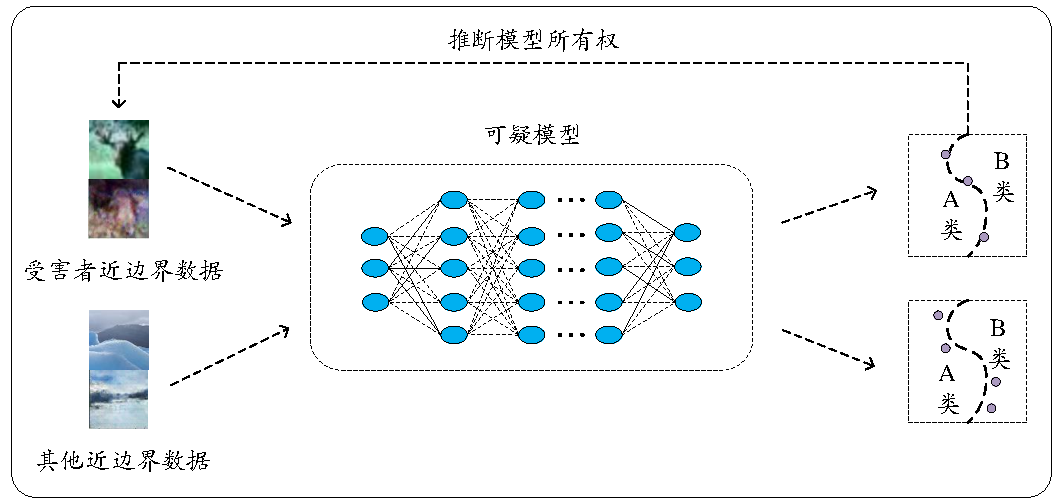
\includegraphics[width=15cm,height=7cm]{方法原理图}
%	\centerline{原始样本}
	\setlength{\abovecaptionskip}{5mm} %图片标题与图片距离
	\caption{近边界数据推断所有权}
	\label{方法原理图}
\end {figure}

\subsection{设计目标}

依据现有的工作,我们的方法在模型训练后进行部署,且在黑盒环境中推断所有权。我们的方法不关注模型盗窃的过程,目的是准确推断受害者所有权和识别可疑模型的盗窃行为。现在大多数所有权验证技术都是黑盒模型环境,因为模型所有者和攻击者通常不会提供完整模型。我们提出的方法仅利用模型提供的外部API,获取近边界数据的决策结果,从而推断模型所有权。在通常的假设中,存在一个官方的仲裁机构,当对任一模型产生所有权怀疑时,受害者和可疑对手可以向机构提出申请并提供各自的私有化近边界数据,并通过我们的方法推断所有权。注意无论在白盒和黑盒的环境中,我们的方法均可以产生效果。

为了实现推断模型所有权,本文提出的方法的设计目标是:
\begin{enumerate}
	\renewcommand{\labelenumi}{\theenumi)}
	\item \textbf{精确性:} 推断模型所有权的方法不应该影响模型的性能,模型的最大可接受测试精度下降不超过5\%。
	\item \textbf{数据近边界性:}如果可疑模型与源模型相同或来自源模型,则根据源模型构造的私有近边界数据在推断模型所有权中距离指定的分类边界最近。
	\item \textbf{鲁棒性:}近边界数据应该对常见的模型修改(如模型微调、剪枝和有损压缩)具有鲁棒性。
	\item \textbf{不可见性:}敌手无法获得私有的近边界数据,也无法在视觉上观察到近边界数据的部署。
	\item \textbf{有效性:}通过近边界数据推断模型所有权应能有效地计算距离边界数据,并通过对比全部近边界数据的决策结果确定可疑模型是盗窃模型。
\end{enumerate}

\subsection{方法概述}

为了实现以上目标,本文提出了一种基于近边界数据的模型所有权推断方法。

\noindent\textbf{问题定义:}我们定义了一个深度神经网络(DNN)分类器$G$作为源模型,给定一个原始训练集$D$,假设该源模型是一个$n$-类的DNN分类器,分类器的输出层为softmax层或其他决策层,决策函数$g_j(x)$表示数据样本$x$被分到第$j$类的概率,其中$j$ = 1,2,..,$n$。$Z_1$,$Z_2$,..,$Z_n$表示模型分类器的全部决策函数输出,其结果可作为分类边界的依据被我们使用,因此

\begin{equation}
	g_j(x) = \frac{exp(Z_j(x))}{\sum_{i = 1}^n exp(Z_i(x))}
\end{equation}

\noindent 其中,数据样本$x$的标签$y$被推断拥有最大概率的类别,例如$y = arg \mathop{max} \limits_j g_j(x) = arg \mathop{max} \limits_j Z_j(x)$。

\begin{myDef}
	\label{def:2}
	\pmb{分类边界}。分类器的分类边界是一个抽象的概念,我们无法直接描述它。因此我们使用分类器的决策结果来反映分类边界。
\end{myDef}

通常来说,寻找位于分类边界上的数据点采用重复随机采样数据点的方法,具体地如果数据点满足上述定义则数据点在分类边界上。然而,简单的重复采样可能需要大量的时间消耗,甚至无法找到这样的数据点们。为了解决这样的问题,我们在\ref{3}中讨论了如何构造位于分类边界上或其附近的的数据点,且将其私有化的过程。

基于\ref{3}的讨论,我们提出构造近边界数据推断模型的所有权,而不是验证所有权。具体而言,如图\ref{方法流程图}所示,我们的方法包括三个主要阶段:
\begin{enumerate}
	\renewcommand{\labelenumi}{\theenumi)}
	\item 从数据集样本中生成对抗性样本;
	\item 训练生成对抗模型生成私有化的近边界数据;
	\item 加入近边界数据微调源模型。
\end{enumerate}

\begin{figure}[htbp]%%图,[htbp]是浮动格式
	\centering
	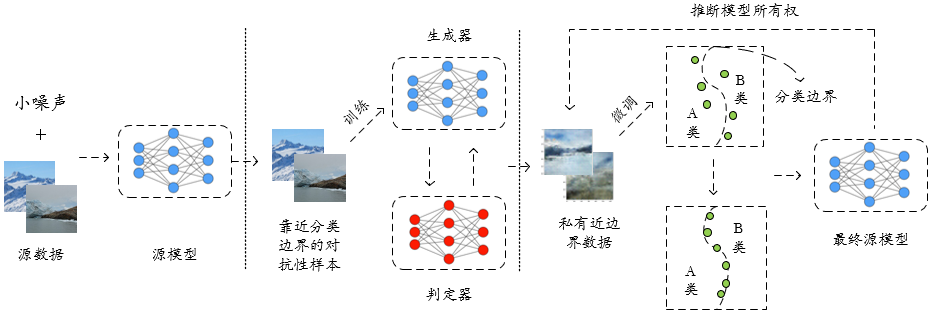
\includegraphics[width=15cm,height=7cm]{方法流程图.png}
	%	\centerline{原始样本}
	\setlength{\abovecaptionskip}{5mm} %图片标题与图片距离
	\caption{方法整体流程图}
	\label{方法流程图}
\end {figure}

\subsection{假设检验}

根据\ref{4}\ref{4.1}讨论的结果,本文认为过去的验证模型所有权的思路具有较大的局限性,大多数研究无法抵御歧义攻击。因此,我们提出了推断模型所有权的想法,这是一种“最”的思路。在现实情况中,我们假设存在第三方仲裁机构,并约定目标分类边界,被盗窃者向第三方机构提出仲裁并提供近边界数据,盗窃者同样需要提供相应的近边界数据,第三方机构分别计算目标分类边
界距离,本文认为持有最靠近目标分类边界的近边界数据所有者将获得模型所有权。注意由于近边界数据通常是一组数据,所以应该根据统计的结果来看。在实践中,我们计算了不同规模的近边界数据组在源模型, 盗窃模型和不相关模型上与分类边界的距离,并设计了一种基于假设检验的方法来表现推断置信度。

\noindent\textbf{假设检验:}我们假设事件$C$是模型所有者提供的私有近边界数据在怀疑模型上的计算结果,事件$C_S$ 表示盗窃者提供的近边界数据在怀疑模型上的计算结果,或模型所有者提供的私有近边界数据在无关模型上的计算结果。本文计算假设$H_0:\mu > \mu_S(H_1:\mu\leq\mu_S)$的$p$值,以及差异大小$\Delta \mu = \mu_S - \mu$,$\Delta\mu$越大,推断可信度越高。如果$p$值低于预定义的置信度评分$\alpha$,则拒绝$H_0$,并称正在测试的模型是被盗模型。我们重复30次统计性实验以提高可信度。


\begin{algorithm}[htbp]
	\setstretch{1.2}
	\caption{InitialDistribution}
	\label{alg:1}
	\begin{algorithmic}[1]
		
		\Require $Nodes,kFrags,Set$
		\Ensure $targetnodes$
		\State $Nodes \gets$ the neighboring online nodes
		\State $kFrags \gets$ the N re-encryption keys the node has generated
		\State $Set \gets$ the set of the nodes that have got the kFrag
		\State $flag \gets$ 0
		\For {$kFrag$ in $kFrags$}
		\State
		\Call{SelectNode}{$Nodes,kFrag,Set,underload$}
		\If{$flag==0$}
		\State \Call{SelectNode}{$Nodes,kFrag,Set,normal$}
		\EndIf
		\If{$flag==0$}
		\State \Call{SelectNode}{$Nodes,kFrag,Set,overload$}
		\EndIf
		\EndFor
		
		
		\State    
		\Function{SelectNode}{$Nodes,kFrag,Set,State$}
		\For{$node$ in $Nodes$}
		\If {$node's$ $state$ is $State$ and $node$ $\notin$ $Set$}
		\State $Send(kFrag)$
		\State $Set=Set \cup node$
		\If{$Size(Set)==Size(Map)$}
		\State $Clear(Set)$
		\EndIf
		\State $flag \gets 1$
		\State $Break$
		
		
		\EndIf
		\EndFor
		\EndFunction
		
		
	\end{algorithmic}
\end{algorithm}

\section{本章小结}

本章从所有权验证的局限性出发,引出了数据集推断,然后详细介绍了近边界数据推断模型所有权的设计目标以及具体的方法流程。


% !TeX root = ../main.tex
% -*- coding: utf-8 -*-

\chapter{基于近边界数据的模型所有权推断方法分析}\label{5}

我们在开源数据集CIFAR-10\cite{krizhevsky2009learning},Heritage\cite{Heritage},Intel\_image\cite{Intel_image}上面进行实验,并选择ResNet18作为评估的源模型,VGG11作为对照的无关模型。本文使用的模型均在开源的预训练模型上进行训练。

\noindent\textbf{被盗模型:}我们设置了常见的几种模型盗窃方法,包括模型微调,模型剪枝(不同的剪枝率)和模型蒸馏,并在源模型的基础上得到被盗模型。

\section{实验设置}\label{5.1}

本文实验利用CIFAR-10,Heritage和Intel\_image三种数据集训练ResNet18,训练过程中Adam优化器并将学习率(Learning rate),迭代轮次(Epoch)和每批次大小(Batch size)分别设置为0.0001,200和64。蒸馏模型实验选择从Resnet18蒸馏至VGG11,蒸馏时将蒸馏温度设置为20并且教师模型比例$\alpha$=0.7,训练轮次是20。初始近边界数据生成采用$CW$-$L_2$算法,实验中选择有目标的生成方式,且学习率,迭代次数和二分搜索次数分别设置为0.001,1000和6,其他参数为默认值。私有近边界数据生成器采用DCGAN的基础结构,训练过程使用Adam优化器且将学习率,训练轮次和每批次大小分别设置为0.0002,8000和64。注意本发明最后微调源模型阶段需要交替使用源模型损失函数和微调目标边界的损失函数来微调源模型,具体设置为10个轮次交替一次且交替次数最多为10次。



\section{生成初始近边界数据的算法选择}\label{5.2}

本小节将对\ref{3}\ref{3.2}中提出的FGSM,IGSM,RFGSM和CW-$L_2$进行测试,我们均使用原作者发布的实现。FGSM,IGSM,RFGSM中均有一个用于界定噪声$\epsilon$的参数,且IGSM和RFGSM还包含一个重要的参数$\alpha$ 用来表示迭代次数。我们进行大量的实验探索选择合适的参数用于与CW-$L_2$进行比较。此外,CW-$L_2$的实验设置如\ref{5.1}所示。如表\ref{table:1}所示,CW-$L_2$生成的对抗性样例与目标分类边界的平均距离远比其他算法小。因此,本文使用该算法作为初始近边界数据生成算法。

\begin{table}[H]
	\centering
	\setlength{\arrayrulewidth}{0.5mm}
	\renewcommand\arraystretch{1.5}
	\caption{不同对抗性样本生成算法生成的数据与目标分类边界的平均距离}
	\label{table:1}
	\begin{tabular*}{13cm}{@{\extracolsep{\fill}} l c c c c}
		
		\hline
		数据集                    &   FGSM   &   IGSM   &  RFGSM  &   CW-$L_2$    \\
		\hline
\multirow{3}{6em}{CIFAR-10}      &    0.557  &   0.430  &  0.418   &    0.066     \\
		                         &    0.461  &   0.419  &  0.373   &    0.103     \\
		                         &    0.586  &   0.369  &  0.356   &    0.112     \\
		\hline
\multirow{3}{6em}{Heritage}      &    0.347  &   0.356  &  0.314   &    0.014     \\
		                         &    0.277  &   0.340  &  0.281   &    0.016     \\
		                         &    0.348  &   0.332  &  0.276   &    0.010     \\
		\hline
\multirow{3}{6em}{Intel\_image}  &    0.522  &   0.447  &  0.353   &    0.088     \\
		                         &    0.475  &   0.506  &  0.387   &    0.122     \\
		                         &    0.468  &   0.402  &  0.428   &    0.127     \\
		\hline		
	\end{tabular*}
\end{table}


\section{数据近边界特性的评估与扩展}\label{5.3}

\begin{figure}[htbp]%%图,[htbp]是浮动格式
	\centering
	\begin{minipage}[htbp]{0.49\linewidth}        %图片占用一行宽度的50%
		\hspace{2mm}
		\centering
		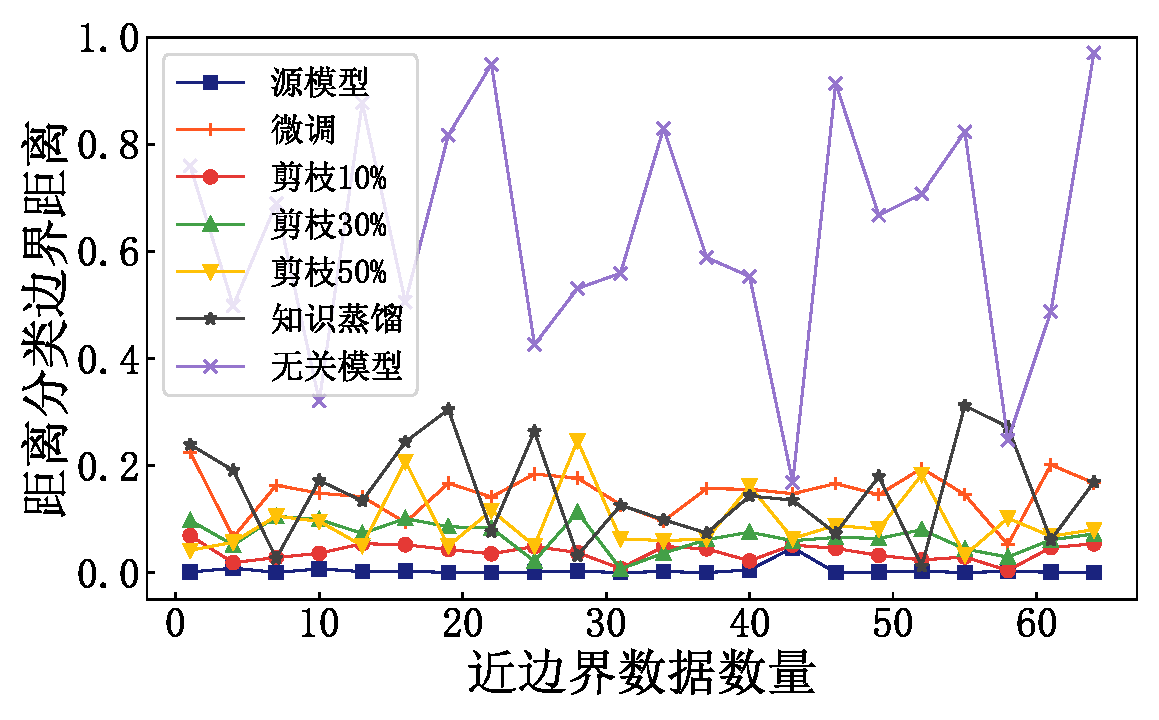
\includegraphics[width=7cm,height=4cm]{CIFAR-10-4-2-distance}
		\centerline{分类边界1}
	\end{minipage}
	\begin{minipage}[htbp]{0.49\linewidth}        %图片占用一行宽度的50%
		\hspace{2mm}
		\centering
		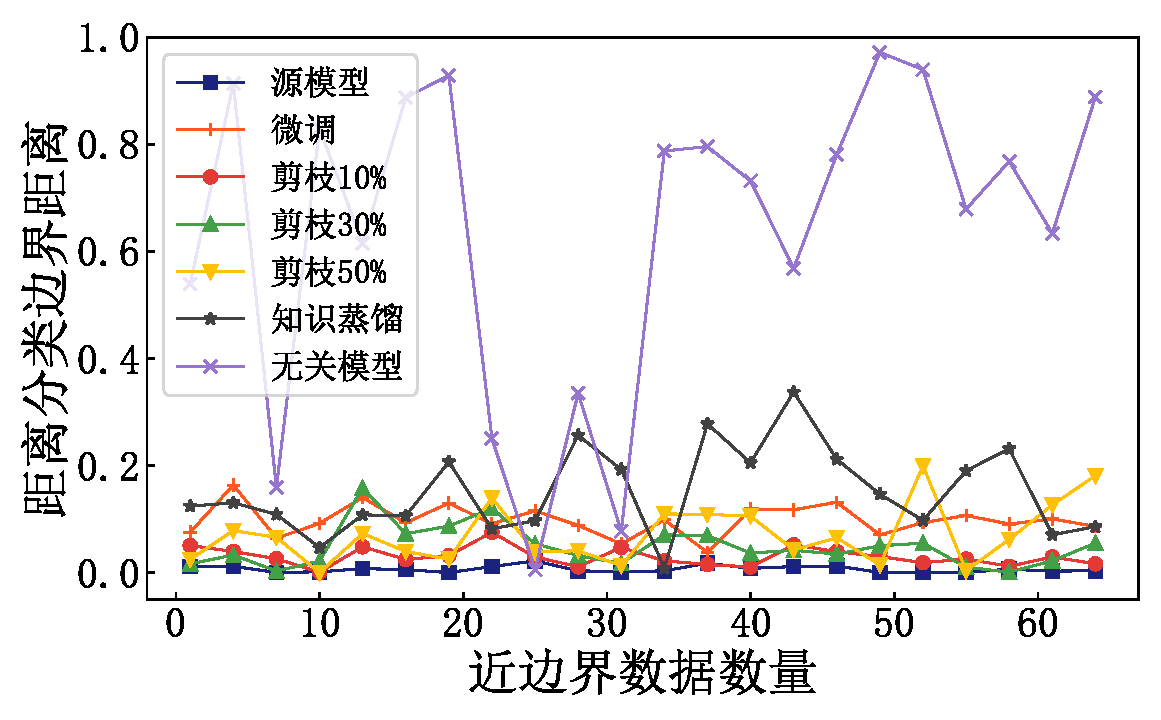
\includegraphics[width=7cm,height=4cm]{CIFAR-10-4-3-distance}
		\centerline{分类边界2}
	\end{minipage}
	\begin{minipage}[htbp]{0.49\linewidth}        %图片占用一行宽度的50%
		\hspace{2mm}
		\centering
		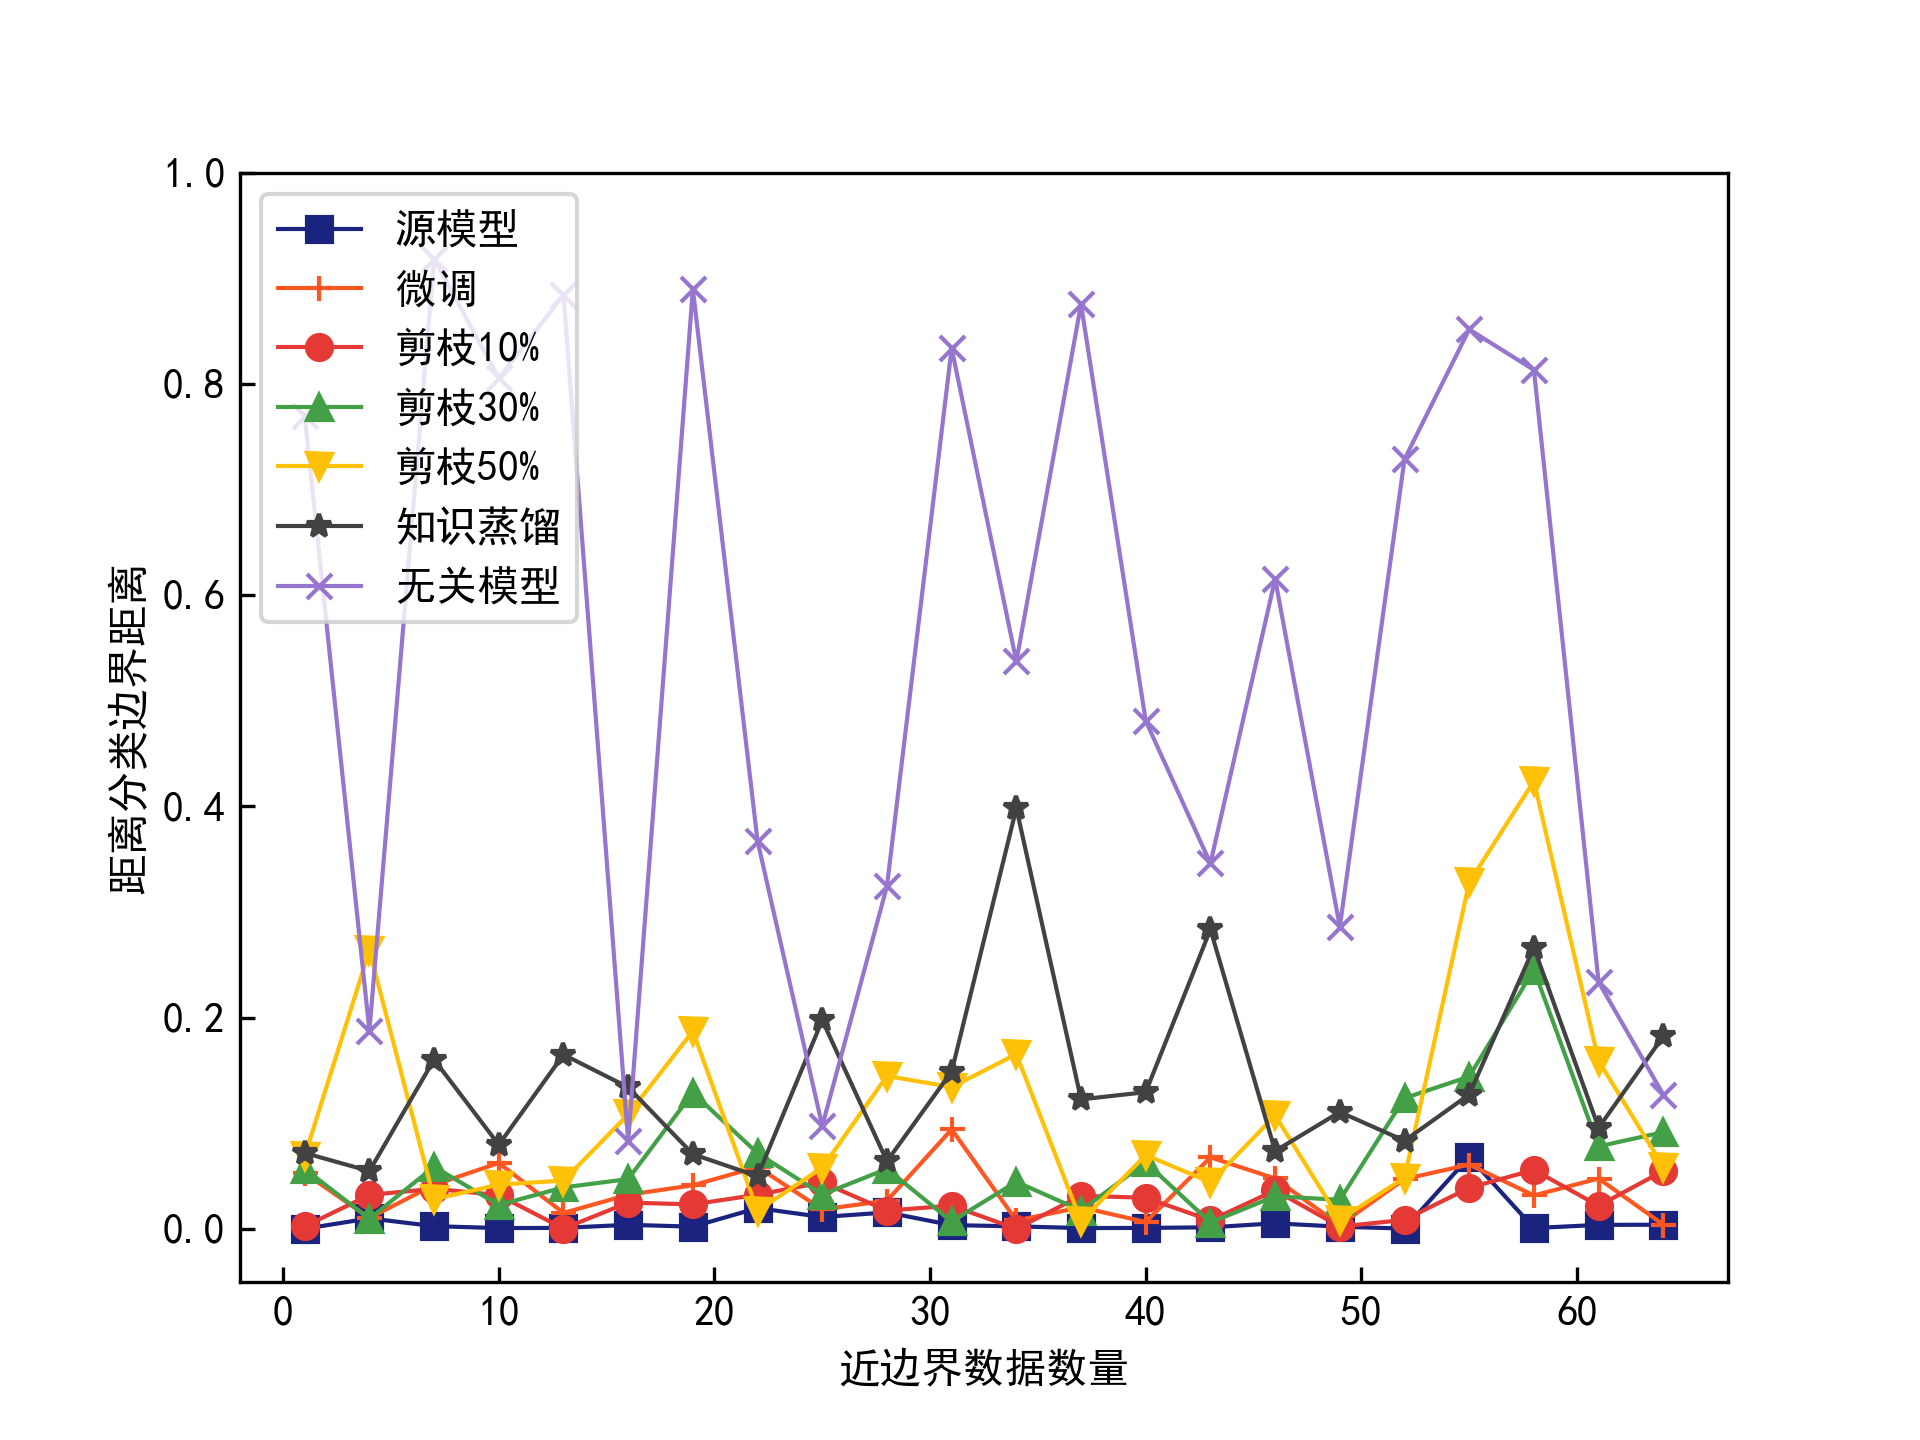
\includegraphics[width=7cm,height=4cm]{CIFAR-10-4-7-distance}
		\centerline{分类边界3}
	\end{minipage}
	\begin{minipage}[htbp]{0.49\linewidth}        %图片占用一行宽度的50%
		\hspace{2mm}
		\centering
		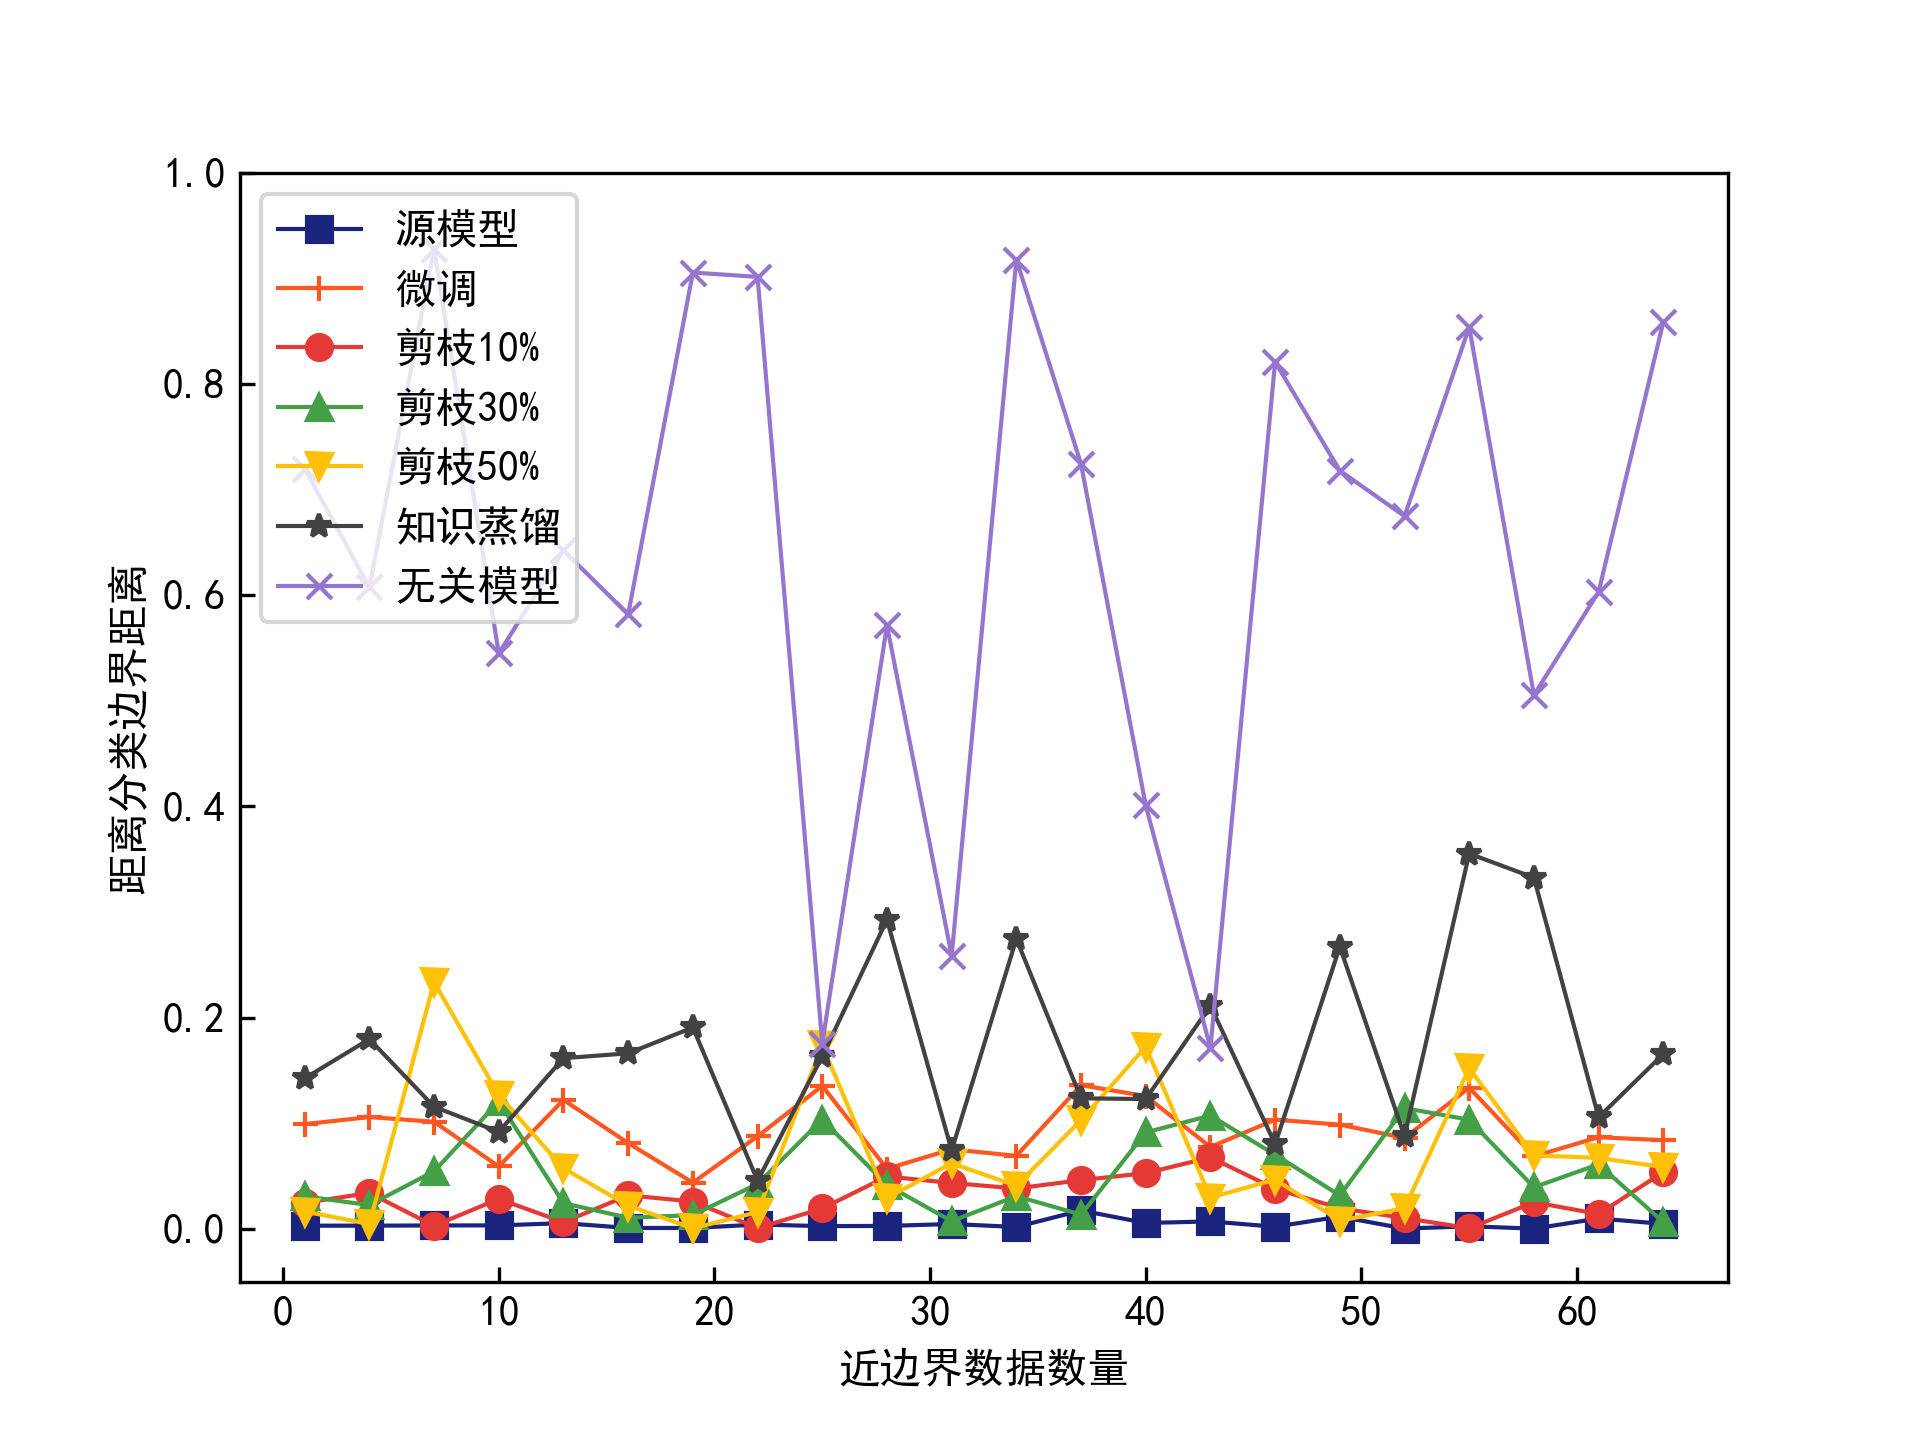
\includegraphics[width=7cm,height=4cm]{CIFAR-10-5-6-distance}
		\centerline{分类边界4}
	\end{minipage}
\setlength{\abovecaptionskip}{7mm} %图片标题与图片距离
\caption{原始样本与对抗性样本对比}
\label{原始样本与对抗性样本对比1}
\end {figure}


\section{推断模型所有权}\label{5.4}

\begin{table}[H]
	\centering
	\setlength{\arrayrulewidth}{0.5mm}
	\renewcommand\arraystretch{1.5}
	\caption{推断模型所有权}
	\label{table:2}
	\resizebox{\linewidth}{!}{
	\begin{tabular}{l l c c c c c c c c c c}
		
		\hline
\multirow{2}{5em}{数据集}&\multirow{2}{4em}{攻击方法}&\multicolumn{2}{c}{分类边界1}&\multicolumn{2}{c}{分类边界2}&\multicolumn{2}{c}{分类边界3}&\multicolumn{2}{c}{分类边界4}&\multicolumn{2}{c}{分类边界5}\\ \cline{3-12}
		                         & &$\Delta\mu$&$p$值&$\Delta\mu$&$p$值&$\Delta\mu$&$p$值&$\Delta\mu$&$p$值&$\Delta\mu$&$p$值 \\
		\hline
\multirow{6}{5em}{CIFAR-10}     &源模型    & 0.913 & $10^{-6}$ & 0.954 & $10^{-6}$ & 0.927 & $10^{-5}$ & 0.967 & $10^{-5}$ & 0.958 & $10^{-5}$   \\
								&模型微调  & 0.718 & $10^{-5}$ & 0.745 & $10^{-6}$ & 0.698 & $10^{-5}$ & 0.692 & $10^{-4}$ & 0.729 & $10^{-5}$   \\
								& 剪枝10\% & 0.572 & $10^{-5}$ & 0.487 & $10^{-5}$ & 0.458 & $10^{-5}$ & 0.533 & $10^{-4}$ & 0.512 & $10^{-4}$   \\
								&剪枝30\%  & 0.537 & $10^{-4}$ & 0.497 & $10^{-4}$ & 0.401 & $10^{-3}$ & 0.428 & $10^{-4}$ & 0.587 & $10^{-4}$   \\
								&剪枝50\%  & 0.545 & $10^{-4}$ & 0.614 & $10^{-4}$ & 0.506 & $10^{-3}$ & 0.570 & $10^{-4}$ & 0.484 & $10^{-3}$   \\
								&知识蒸馏  & 0.372 & $10^{-3}$ & 0.297 & $10^{-3}$ & 0.288 & $10^{-3}$ & 0.308 & $10^{-3}$ & 0.340 & $10^{-3}$   \\
		\hline
\multirow{6}{5em}{Heritage}     &源模型    & 0.876 & $10^{-5}$ & 0.845 & $10^{-5}$ & 0.859 & $10^{-4}$ & 0.801 & $10^{-4}$ & 0.837 & $10^{-5}$   \\
								&模型微调  & 0.815 & $10^{-5}$ & 0.792 & $10^{-4}$ & 0.824 & $10^{-4}$ & 0.833 & $10^{-4}$ & 0.784 & $10^{-4}$   \\
								&剪枝10\%  & 0.530 & $10^{-4}$ & 0.535 & $10^{-3}$ & 0.508 & $10^{-4}$ & 0.486 & $10^{-3}$ & 0.471 & $10^{-3}$   \\
								&剪枝30\%  & 0.491 & $10^{-3}$ & 0.452 & $10^{-3}$ & 0.469 & $10^{-4}$ & 0.470 & $10^{-3}$ & 0.427 & $10^{-4}$   \\
								&剪枝50\%  & 0.502 & $10^{-3}$ & 0.517 & $10^{-3}$ & 0.434 & $10^{-3}$ & 0.451 & $10^{-3}$ & 0.490 & $10^{-3}$   \\
								&知识蒸馏  & 0.329 & $10^{-3}$ & 0.365 & $10^{-2}$ & 0.238 & $10^{-3}$ & 0.310 & $10^{-3}$ & 0.274 & $10^{-3}$   \\
		\hline
\multirow{6}{5em}{Intel\_image} &源模型    & 0.859 & $10^{-5}$ & 0.896 & $10^{-4}$ & 0.872 & $10^{-4}$ & 0.899 & $10^{-4}$ & 0.914 & $10^{-4}$   \\
								&模型微调  & 0.717 & $10^{-5}$ & 0.784 & $10^{-4}$ & 0.752 & $10^{-4}$ & 0.791 & $10^{-3}$ & 0.709 & $10^{-4}$   \\
								&剪枝10\%  & 0.451 & $10^{-4}$ & 0.522 & $10^{-4}$ & 0.539 & $10^{-3}$ & 0.472 & $10^{-3}$ & 0.438 & $10^{-4}$   \\
								&剪枝30\%  & 0.407 & $10^{-4}$ & 0.415 & $10^{-4}$ & 0.346 & $10^{-3}$ & 0.382 & $10^{-3}$ & 0.395 & $10^{-3}$   \\
								&剪枝50\%  & 0.370 & $10^{-3}$ & 0.395 & $10^{-3}$ & 0.327 & $10^{-3}$ & 0.360 & $10^{-3}$ & 0.458 & $10^{-3}$   \\
								&知识蒸馏  & 0.336 & $10^{-2}$ & 0.395 & $10^{-3}$ & 0.360 & $10^{-2}$ & 0.308 & $10^{-3}$ & 0.287 & $10^{-2}$   \\
		\hline		
	\end{tabular}
}
\end{table}



\section{微调目标分类边界的影响}\label{5.5}

\begin{table}[H]
	\centering
	\setlength{\arrayrulewidth}{0.5mm}
	\renewcommand\arraystretch{1.8}
	\caption{微调分类边界对模型的影响}
	\label{table:state}
	\begin{tabular*}{13cm}{@{\extracolsep{\fill}} l c c}
		
	\hline
	数据集        &    微调前准确率   &   微调后准确率            \\
	\hline
	CIFAR-10      &     0.886        &     0.873               \\
	
	Heritage      &     0.879        &     0.856               \\
	
	Intel\_image  &     0.794        &     0.786               \\
	\hline		
	\end{tabular*}
\end{table}

\begin{table}[H]
	\centering
	\setlength{\arrayrulewidth}{0.5mm}
	\renewcommand\arraystretch{1.2}
	\caption{CIFAR-10上不同对抗性样本生成算法生成的数据与目标分类边界的平均距离}
	\label{table:3}
	\begin{tabular*}{14cm}{@{\extracolsep{\fill}} l l c c}
		
		\hline
		数据集 \ (准确率)   &   分类边界   &  数据数量  &   微调后准确率    \\
		\hline
\multirow{20}{8em}{CIFAR-10\ (0.886)}         &\multirow{4}{6em}{分类边界1}&  64   & 0.873    \\
								              &                           &  128  & 0.862     \\
								              &                           &  256  & 0.862     \\
								              &                           &  512  & 0.854     \\
		\cline{2-4}						   
								              &\multirow{4}{6em}{分类边界2} &  64  & 0.871 \\
								              &                            &  128 & 0.870     \\
								              &                            &  256 & 0.860     \\
								              &                            &  512 & 0.844     \\
		
		\cline{2-4}						       
											  &\multirow{4}{6em}{分类边界3} & 64   & 0.871  \\
											  &                            &  128 & 0.868     \\
											  &                            &  256 & 0.858     \\
											  &                            &  512 & 0.856     \\
		\cline{2-4}						       
											  &\multirow{4}{6em}{分类边界4} & 64   & 0.873  \\
											  &                            &  128 & 0.873     \\
											  &                            &  256 & 0.866     \\
											  &                            &  512 & 0.862     \\
		\cline{2-4}						       
											  &\multirow{4}{6em}{分类边界5} & 64  & 0.876  \\
											  &                            & 128 & 0.866     \\
											  &                            & 256 & 0.868     \\
											  &                            & 512 & 0.861     \\
		\hline	
	\end{tabular*}
\end{table}

\begin{table}[H]
	\centering
	\setlength{\arrayrulewidth}{0.5mm}
	\renewcommand\arraystretch{1.2}
	\caption{Heritage上不同对抗性样本生成算法生成的数据与目标分类边界的平均距离}
	\label{table:4}
	\begin{tabular*}{14cm}{@{\extracolsep{\fill}} l l c c}
		
		\hline
		数据集 \ (准确率)   &   分类边界   &  数据数量  &   微调后准确率    \\
		\hline
		\multirow{20}{8em}{Heritage\ (0.879)}         &\multirow{4}{6em}{分类边界1}&  64   & 0.856    \\
		&                           &  128  & 0.825     \\
		&                           &  256  & 0.830     \\
		&                           &  512  & 0.797     \\
		\cline{2-4}						   
		&\multirow{4}{6em}{分类边界2} &  64  & 0.823 \\
		&                            &  128 & 0.839     \\
		&                            &  256 & 0.841     \\
		&                            &  512 & 0.779     \\
		
		\cline{2-4}						       
		&\multirow{4}{6em}{分类边界3} & 64   & 0.848  \\
		&                            &  128 & 0.826     \\
		&                            &  256 & 0.779     \\
		&                            &  512 & 0.791     \\
		\cline{2-4}						       
		&\multirow{4}{6em}{分类边界4} & 64   & 0.819  \\
		&                            &  128 & 0.795     \\
		&                            &  256 & 0.803     \\
		&                            &  512 & 0.783     \\
		\cline{2-4}						       
		&\multirow{4}{6em}{分类边界5} & 64  & 0.843  \\
		&                            & 128 & 0.851     \\
		&                            & 256 & 0.776     \\
		&                            & 512 & 0.774     \\
		\hline	
	\end{tabular*}
\end{table}

\begin{table}[H]
	\centering
	\setlength{\arrayrulewidth}{0.5mm}
	\renewcommand\arraystretch{1.2}
	\caption{Intel\_image上不同对抗性样本生成算法生成的数据与目标分类边界的平均距离}
	\label{table:5}
	\begin{tabular*}{14cm}{@{\extracolsep{\fill}} l l c c}
		
		\hline
		数据集 \ (准确率)   &   分类边界   &  数据数量  &   微调后准确率    \\
		\hline
		\multirow{20}{8em}{Intel\_image\ (0.794)}    &\multirow{4}{6em}{分类边界1}&  64   & 0.755    \\
		&                           &  128  & 0.769     \\
		&                           &  256  & 0.756     \\
		&                           &  512  & 0.779     \\
		\cline{2-4}						   
		&\multirow{4}{6em}{分类边界2} &  64  & 0.770 \\
		&                            &  128 & 0.741     \\
		&                            &  256 & 0.768     \\
		&                            &  512 & 0.777     \\
		
		\cline{2-4}						       
		&\multirow{4}{6em}{分类边界3} & 64   & 0.781  \\
		&                            &  128 & 0.753     \\
		&                            &  256 & 0.764     \\
		&                            &  512 & 0.752     \\
		\cline{2-4}						       
		&\multirow{4}{6em}{分类边界4} & 64   & 0.787  \\
		&                            &  128 & 0.751     \\
		&                            &  256 & 0.762     \\
		&                            &  512 & 0.747     \\
		\cline{2-4}						       
		&\multirow{4}{6em}{分类边界5} & 64  & 0.786  \\
		&                            & 128 & 0.764     \\
		&                            & 256 & 0.761     \\
		&                            & 512 & 0.765     \\
		\hline	
	\end{tabular*}
\end{table}

\section{可伸缩性扩展}\label{5.6}




\section{本章小结}
% !TeX root = ../main.tex
% -*- coding: utf-8 -*-
\chapter{总结与展望}\label{6}


\section{工作总结}


\section{工作展望}

%%%%%%%%%%%%%%%%%%%%%%%%%%%%
% 论文其他信息
%%%%%%%%%%%%%%%%%%%%%%%%%%%%
% !TeX root = ../main.tex
% -*- coding: utf-8 -*-

\printbibliography

% !TeX root = ../main.tex
% -*- coding: utf-8 -*-

% !TeX root = ../main.tex
% -*- coding: utf-8 -*-

%\makeschapterhead{致谢}
\chapter*{致谢}
谢谢。

% !TeX root = ../main.tex
% -*- coding: utf-8 -*-

\chapter*{个人简历}


xxx,出生于yyyy年mm月dd日。
在20yy年毕业于xx大学XX专业并获得xx士学位。
于20xx年至今在南开大学就读xxx研究生。


\section*{\leftline{研究生期间发表论文:}}
% 学术论文研究成果按发表的时间顺序列出
% (已发表的列在前面,已接收待发表的放在后面)
% 格式方便阅读为主可参考百度学术Google学术

\begin{itemize}
	\item 周恩来. 周恩来选集[M]. 人民出版社, 1980.
	\item 周恩来. 周恩来外交文选[M]. 中央文献出版社, 1990.
\end{itemize}




% 其他成果有可添加
% \section*{\leftline{研究生期间其它成果:}}
% % 研究成果可以是在学期间参加的研究项目、申请的专利或获奖等
% \begin{itemize}
% 	\item 
% \end{itemize}


\end{document}
